\chapter{Perkembangan Lembaga Vertebrata}\label{ch:b2:vertebrate-development}

Sebutir telur katak adalah sebuah bola bergaris tengah dua milimeter,
gelap di atas dan pucat di bawah. Dalam sehari ia telah membelah
menjadi ribuan sel; dalam dua hari, sehelai lembaran sel itu telah
bergulir masuk lewat sebuah alur untuk membuat sebuah usus lalu
meletakkan sebatang tongkat sepanjang punggungnya; dalam tiga hari,
lembaran di atas tongkatnya telah melipat menjadi sebuah tabung yang
akan menjadi otak dan sumsum tulang belakangnya. Tidak ada yang
ditambahkan kecuali air. Keterangan yang mengubah satu sel menjadi
seekor berudu yang berenang sudah ada di dalam telurnya dan genomnya,
dan cara ia terbuka --- pembelahan, gastrulasi, neurulasi, pengimbasan
tiap bagiannya oleh tetangganya --- dapat dikenali sama pada seekor
ikan, seekor anak ayam, dan seekor mencit. Bab ini mengikuti sebuah
lembaga vertebrata melalui langkah itu lalu memerikan percobaan yang
menunjukkan bagaimana tiap bagiannya diberi tahu akan menjadi apa.

\section{Dari telur ke blastula}

\begin{definition}[Telur dan sumbunya]\label{def:b2:vertebrate-development:egg}
\index{kutub hewan}\index{kutub tumbuhan}\index{kuning telur}\index{pembelahan}
Sebutir telur vertebrata sudah terkutub sebelum pembuahan:
\emph{kutub hewan}nya memuat nukleus dan sebagian besar sitoplasmanya,
\emph{kutub tumbuhan}nya memuat \emph{kuning telur}, yaitu simpanan
protein dan lipid yang menghidupi lembaganya sampai ia makan. Banyaknya
kuning telur menetapkan pola segala yang menyusul: telur bulu babi laut
atau mamalia hampir tidak memilikinya dan membelah sepenuhnya menjadi
sel yang sama besar; telur katak memilikinya dalam jumlah sedang dan
membelah sepenuhnya tetapi tidak sama besar (sel kecil di atas, sel
besar berkuning telur di bawah); telur ikan atau burung hampir
seluruhnya kuning telur dan hanya membelah pada sebuah cakram
sitoplasma di atasnya. Pada katak, titik masuk spermanya menetapkan
sumbu keduanya: korteksnya berputar tiga puluh derajat menjauhinya lalu
menyingkapkan sebuah \emph{sabit kelabu} berseberangan dengan titik
masuknya, dan sisi itu akan menjadi punggungnya. \emph{Pembelahan}
adalah serangkaian mitosis cepat tanpa pertumbuhan --- selnya memeroh
ukurannya tiap kalinya --- yang digerakkan mRNA dan protein dari
induknya yang tersimpan di dalam telurnya, sedangkan gen lembaganya
sendiri tetap membisu sampai \emph{peralihan \omterm{def:b2:vertebrate-development:blastula}{blastula}
tengah}, kira-kira dua belas pembelahan kemudian.
\end{definition}

\begin{omfigure}
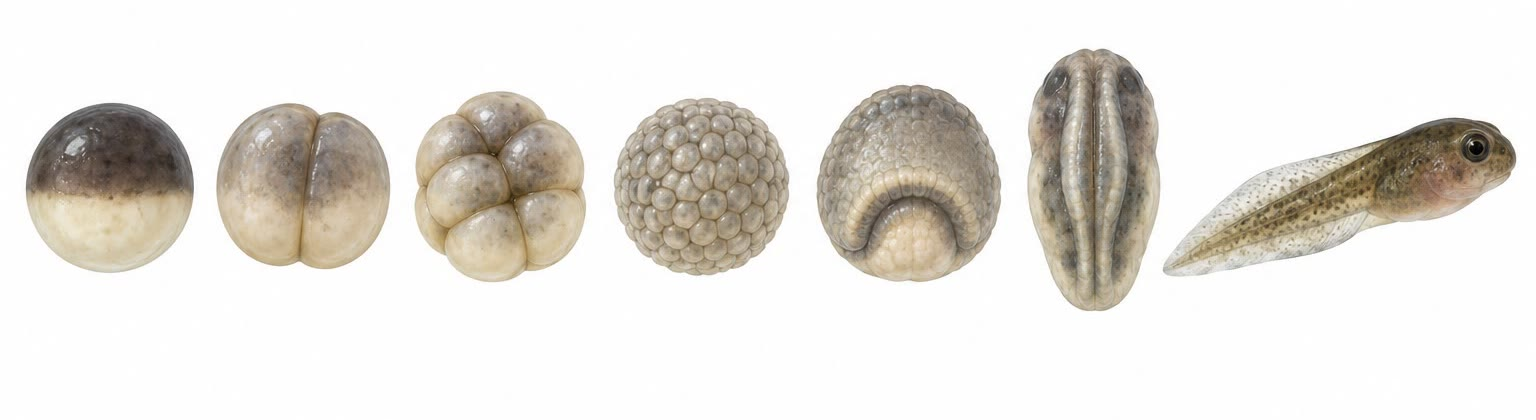
\includegraphics[width=0.9\linewidth]{images/book4/ai/b4-10-frog-development.jpg}

{\small Perkembangan seekor katak dari telur yang telah dibuahi:
pembelahan sampai sebuah \omterm{def:b2:vertebrate-development:blastula}{blastula}, gastrulasi, neurula dengan lipatan
sarafnya, dan berudunya --- semuanya dalam beberapa hari, tanpa
pertumbuhan.}
\end{omfigure}

\begin{theorem}[Aritmetika pembelahan]\label{thm:b2:vertebrate-development:cleavage}
Sesudah $k$ pembelahan serentak, sebutir telur bervolume $V_0$ menjadi
$2^{k}$ sel yang purata volumenya $V_0/2^{k}$ dan jari-jarinya
$r_0/2^{k/3}$, dan seluruh permukaannya telah tumbuh dengan $2^{k/3}$;
rasio volume nukleus terhadap volume sitoplasmanya, yang bermula
mendekati $10^{-4}$ pada sebutir telur katak, naik dengan $2^{k}$ lalu
mencapai rasio sebuah sel biasa ($\sim 0.1$) sesudah kira-kira sepuluh
pembelahan. Rasio yang naik inilah --- penitaran sebuah persediaan
penghambat tetap dari induknya oleh jumlah DNA yang tumbuh secara
eksponensial --- yang memicu peralihan \omterm{def:b2:vertebrate-development:blastula}{blastula} tengah:
pembelahannya melambat, menjadi tak serentak, dan genom zigotiknya
menyala.
\end{theorem}
\begin{proof}
Volumenya kekal pada pembelahan, sehingga masing-masing dari $2^{k}$
selnya memiliki $V_0
2^{-k}$ dan, sebagai sebuah bola, jari-jari $r_0 2^{-k/3}$; seluruh
luasnya adalah
$2^{k}\cdot 4\pi r_0^{2}\, 2^{-2k/3} = 4\pi r_0^{2}\, 2^{k/3}$. Tiap
selnya menyimpan satu nukleus berukuran tetap, sehingga rasionya
berskala $2^{k}$ dari $10^{-4}$: $2^{10} = 1024$ membawanya ke $0.1$.
Peralihan pada katak jatuh pada pembelahan kedua belas, sepadan dengan
sebuah ambang yang tercapai sedikit kemudian.
\end{proof}
\begin{proof}[Bukti eksperimental]
Newport dan Kirschner (1982) menambahkan DNA berlebih ke dalam telur
katak lalu mendapati peralihannya datang lebih awal sebanyak pembelahan
seperti berlebihnya DNA itu; membuang sitoplasmanya memberi pengaruh
yang sama. Jamnya bukanlah waktu atau cacah pembelahan melainkan sebuah
rasio.
\end{proof}

\begin{definition}[Blastula]\label{def:b2:vertebrate-development:blastula}
\index{blastula}\index{blastosol}
Pembelahannya berakhir pada sebuah \emph{blastula}: sebuah bola
berongga (katak, bulu babi laut) atau sebuah cakram (ikan, burung)
berisi beberapa ribu sel mengelilingi sebuah rongga, yaitu
\emph{blastosol}. Selnya masih tak terkhusus penampilannya, tetapi
mereka tidak setara: sebuah \emph{peta nasib}, yang dibuat dengan
mewarnai bercak permukaannya dengan zat warna lalu mengikutinya,
menunjukkan bahwa tudung hewannya akan memberi kulit dan sistem saraf
(\emph{ektoderm}), sabuk khatulistiwanya memberi otot, rangka, ginjal,
dan darah (\emph{mesoderm}), serta massa tumbuhannya memberi usus dan
organnya (\emph{endoderm}). Ketiga \emph{lapisan lembaga} ini sama pada
tiap vertebrata, dan langkah berikutnya adalah menaruhnya pada
tempatnya: mesoderm dan endodermnya berada di luar dan harus masuk.
\end{definition}

\section{Gastrulasi dan neurulasi}

\begin{proposition}[Gastrulasi]\label{prop:b2:vertebrate-development:gastrulation}
\index{gastrulasi}\index{blastopor}\index{arkenteron}\index{notokord}
\emph{Gastrulasi} adalah perangkat gerakan sel yang mengubah \omterm{def:b2:vertebrate-development:blastula}{blastula}
berlapis satu menjadi sebuah \emph{gastrula} berlapis tiga. Pada
kataknya ia mulai di bawah sabit kelabunya: sel di situ berganti
bentuk, mengerutkan ujung luarnya menjadi botol, dan permukaannya
melengkung ke dalam menjadi sebuah alur, yaitu \emph{blastopor}.
Lewatnya mesoderm dan endodermnya mengalir masuk (\emph{involusi}),
bergulir melewati bibirnya lalu bergerak maju sepanjang atap rongganya;
tudung hewannya menyebar turun untuk menutupi bagian luarnya
(\emph{epiboli}); blastopornya menutup menjadi sebuah cincin di
sekeliling sel berkuning telur yang terakhir. Di dalamnya, sebuah
rongga baru yang berlapis endoderm, yaitu \emph{arkenteron}, adalah
bakal ususnya, dan mesoderm yang bergulir masuk lebih dahulu, sepanjang
garis tengahnya, telah menjadi sebatang tongkat kaku, yaitu
\emph{notokord}, yakni sumbu tiap lembaga vertebrata dan struktur yang
menamai filumnya. Pada burung dan mamalia, gerakan yang sama terjadi
lewat sebuah celah, yaitu \emph{garis primitif}, di dalam sebuah cakram
datar; pada ikan cakramnya menyebar di atas \omterm{def:b2:vertebrate-development:egg}{kuning telurnya}.
Koreografinya berbeda menurut \omterm{def:b2:vertebrate-development:egg}{kuning telurnya}; hasilnya --- ektoderm di
luar, endoderm melapisi ususnya, mesoderm di antaranya, notokord pada
garis tengahnya --- tetap sama.
\end{proposition}

\begin{omfigure}
\begin{tikzpicture}[every node/.style={font=\scriptsize}, >=stealth]
  % blastula
  \begin{scope}
    \draw[thick, fill=omDef!15] (0,0) circle (1.3);
    \draw[thick, fill=white] (0,0.2) circle (0.75);
    \fill[omExo!40] (0,0) ++(-1.3,0) arc (180:360:1.3 and 1.3) -- cycle;
    \draw[thick] (0,0) circle (1.3);
    \node at (0,0.2) {blastosol};
    \node[below, align=center] at (0,-1.45) {blastula\\tudung hewan (biru), sel berkuning telur (kelabu)};
  \end{scope}
  % early gastrula: blastopore forming
  \begin{scope}[xshift=4.2cm]
    \draw[thick, fill=omDef!15] (0,0) circle (1.3);
    \draw[thick, fill=white] (0,0.25) circle (0.7);
    \fill[omExo!40] (0,0) ++(-1.3,0) arc (180:360:1.3 and 1.3) -- cycle;
    \draw[thick] (0,0) circle (1.3);
    \draw[very thick, omThm] (1.0,-0.85) .. controls (0.5,-0.6) and (0.4,-0.3) .. (0.55,0.0);
    \draw[->, thick, omThm] (1.15,-0.7) .. controls (0.6,-0.4) .. (0.4,0.1);
    \draw[omThm] (1.0,-0.85) -- (0.9,-1.25); \node[omThm, anchor=north west] at (0.6,-1.2) {bibir blastopor};
    \node[below, align=center] at (0,-1.45) {gastrula dini\\selnya bergulir masuk melewati bibirnya};
  \end{scope}
  % late gastrula
  \begin{scope}[xshift=8.4cm]
    \draw[thick, fill=omDef!15] (0,0) circle (1.3);
    \draw[thick, fill=omExo!25] (0,0.05) circle (0.95);
    \draw[thick, fill=white] (0.15,-0.1) ellipse (0.55 and 0.4);
    \draw (0.6,-0.3) -- (1.6,-1.15); \node[anchor=west] at (1.6,-1.15) {arkenteron};
    \draw[very thick, omThm] (-0.9,0.35) .. controls (-0.2,0.6) .. (0.8,0.4);
    \draw[omThm] (0.0,0.48) -- (-0.9,1.55); \node[omThm, anchor=east] at (-0.9,1.55) {notokord};
    \draw[thick] (1.1,-0.7) -- (1.3,-0.5);
    \node[right] at (1.3,-0.5) {blastopor};
    \node[below, align=center] at (0,-1.45) {gastrula lanjut: tiga lapis,\\rongga usus, notokord pada atapnya};
  \end{scope}
\end{tikzpicture}

{\small Gastrulasi pada katak, dalam potongan. Selnya bergulir ke dalam
melewati bibir blastoporanya; endodermnya melapisi sebuah rongga usus
baru, dan mesoderm yang pertama masuk menjadi notokord sepanjang garis
tengahnya.}
\end{omfigure}

\begin{proposition}[Neurulasi dan rancang bangun tubuhnya]\label{prop:b2:vertebrate-development:neurulation}
\index{neurulasi}\index{tabung saraf}\index{somit}\index{pial saraf}
Ektoderm di atas notokordnya menebal menjadi sebuah \emph{lempeng
saraf}, yang tepinya menjulang sebagai lipatan lalu bertemu pada garis
tengahnya membentuk \emph{\omterm{prop:b2:vertebrate-development:neurulation}{tabung saraf}}, yaitu bakal otak dan sumsum
tulang belakangnya, yang tenggelam di bawah kulitnya; sel dari puncak
lipatannya, yaitu \emph{\omterm{prop:b2:vertebrate-development:neurulation}{pial saraf}}, bermigrasi pergi untuk membuat
saraf tepinya, sel pigmennya, medula adrenalnya, dan sebagian besar
wajahnya. Pada tiap sisi notokordnya, mesodermnya beruas menjadi
bongkah, yaitu \emph{somit}, sepasang demi sepasang dari kepala ke
ekornya, yang memberi ruas tulang belakang, otot batang tubuh, dan
dermisnya; mesoderm sampingnya terbelah menjadi lapisan yang melapisi
rongga tubuhnya serta membuat jantung dan tungkainya; tabung endodermnya
menunaskan paru-paru, hati, dan pankreasnya. Pada akhir neurulasinya,
lembaganya sudah memiliki rancang bangun tubuh vertebrata --- sebuah
tali saraf punggung di atas sebuah notokord, sebuah usus perut, otot
beruas, sebuah kepala --- pada panjang beberapa milimeter, dan sisa
perkembangannya adalah penggarapan organ dari rancangan ini
(\cref{ch:b2:limb-organogenesis}).
\end{proposition}

\begin{omfigure}
\begin{tikzpicture}[every node/.style={font=\scriptsize}]
  \foreach \x/\lab in {0/{lempeng saraf}, 4.0/{lipatan sarafnya menjulang}, 8.0/{tabung saraf menutup; pial saraf bermigrasi}} {
    \begin{scope}[xshift=\x cm]
      \draw[thick, fill=omExo!25] (-1.6,0) rectangle (1.6,-1.6);
      \draw[thick, omThm, fill=omThm!30] (0,-0.75) circle (0.28);
      \draw[thick, fill=omProp!30] (-1.3,-0.75) circle (0.32); \draw[thick, fill=omProp!30] (1.3,-0.75) circle (0.32);
      \node[below, align=center, text width=3.4cm] at (0,-1.7) {\lab};
    \end{scope}
  }
  \draw[very thick, omDef] (-1.6,0) -- (-0.7,0) .. controls (-0.3,0.15) and (0.3,0.15) .. (0.7,0) -- (1.6,0);
  \draw[very thick, omDef] (2.4,0) -- (3.3,0) .. controls (3.3,0.9) and (3.6,0.1) .. (4.0,0.0) .. controls (4.4,0.1) and (4.7,0.9) .. (4.7,0) -- (5.6,0);
  \draw[very thick, omDef] (6.4,0.05) -- (9.6,0.05);
  \draw[very thick, omDef, fill=omDef!20] (8.0,-0.3) circle (0.3);
  \foreach \p in {(7.35,-0.4),(8.65,-0.4)} \fill[omDef!70!black] \p circle (0.07);
  \node[omThm, anchor=west] at (9.8,-0.75) {notokord};
  \node[omProp, anchor=west] at (9.8,-1.15) {somit};
  \node[omDef, anchor=west] at (9.8,-0.3) {tabung saraf};
  \node[omDef!70!black, anchor=west] at (9.8,0.1) {sel pial saraf};
\end{tikzpicture}

{\small Neurulasi dalam potongan melintang: ektoderm di atas
notokordnya (merah) menebal, melipat, lalu menutup menjadi \omterm{prop:b2:vertebrate-development:neurulation}{tabung saraf}
(biru), sementara mesoderm di sebelah notokordnya beruas menjadi
somit (jingga) dan sel \omterm{prop:b2:vertebrate-development:neurulation}{pial saraf} meninggalkan lipatan yang menutup.}
\end{omfigure}

\begin{omfigure}
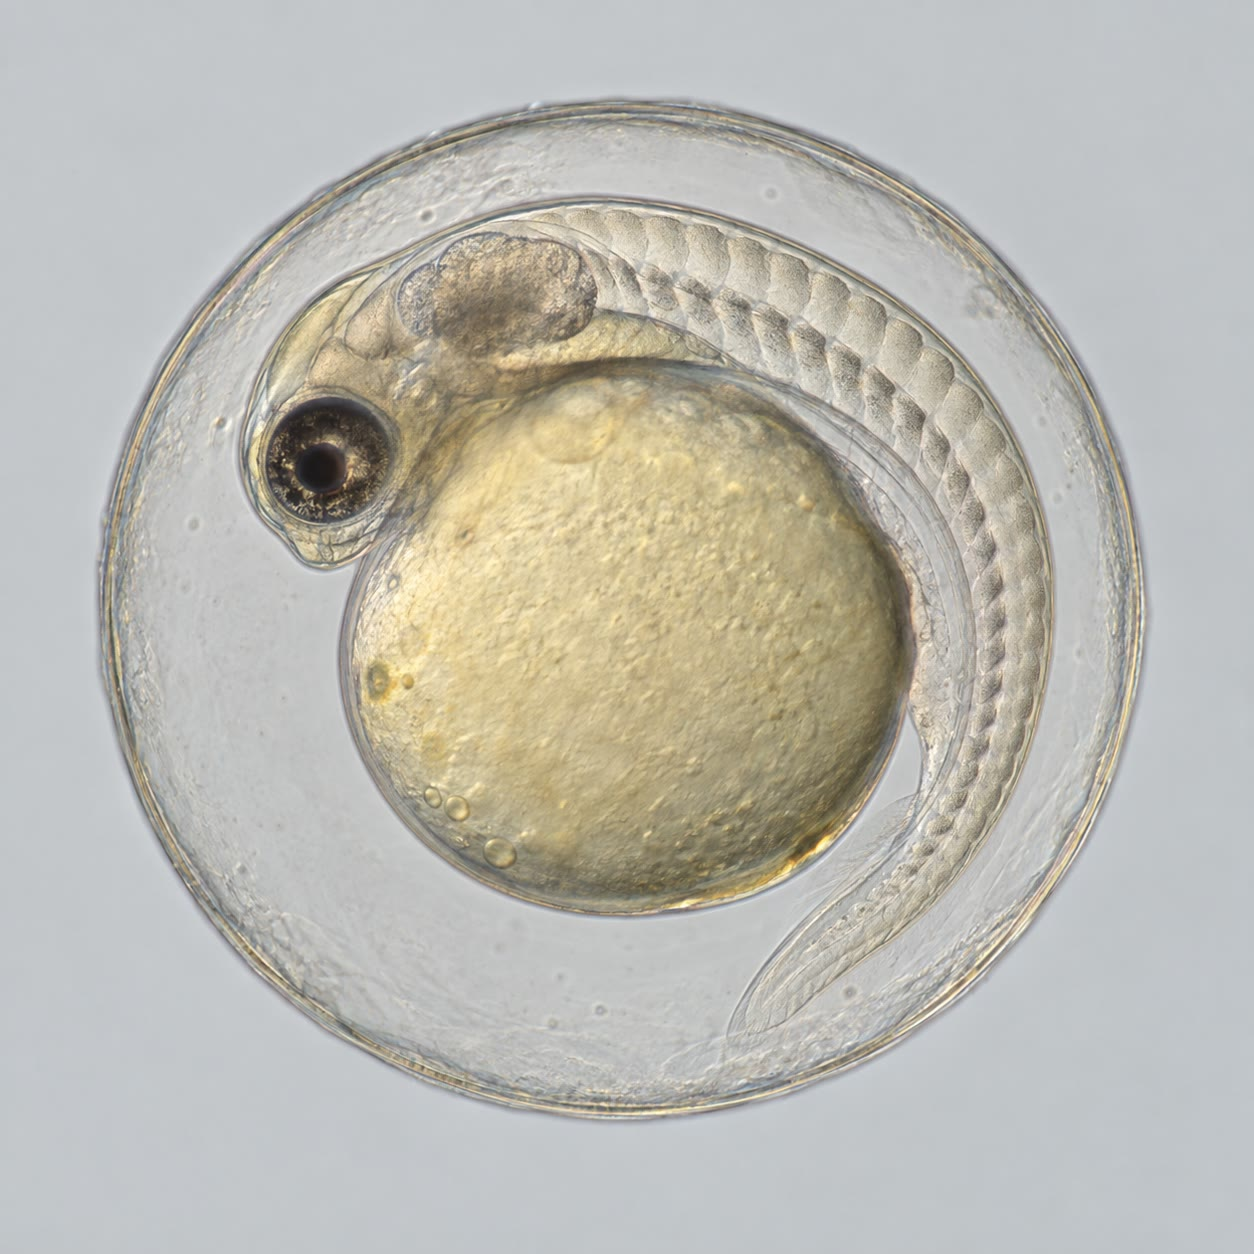
\includegraphics[width=0.42\linewidth]{images/book4/ai/b4-10-zebrafish-embryo.jpg}\hspace{0.04\linewidth}
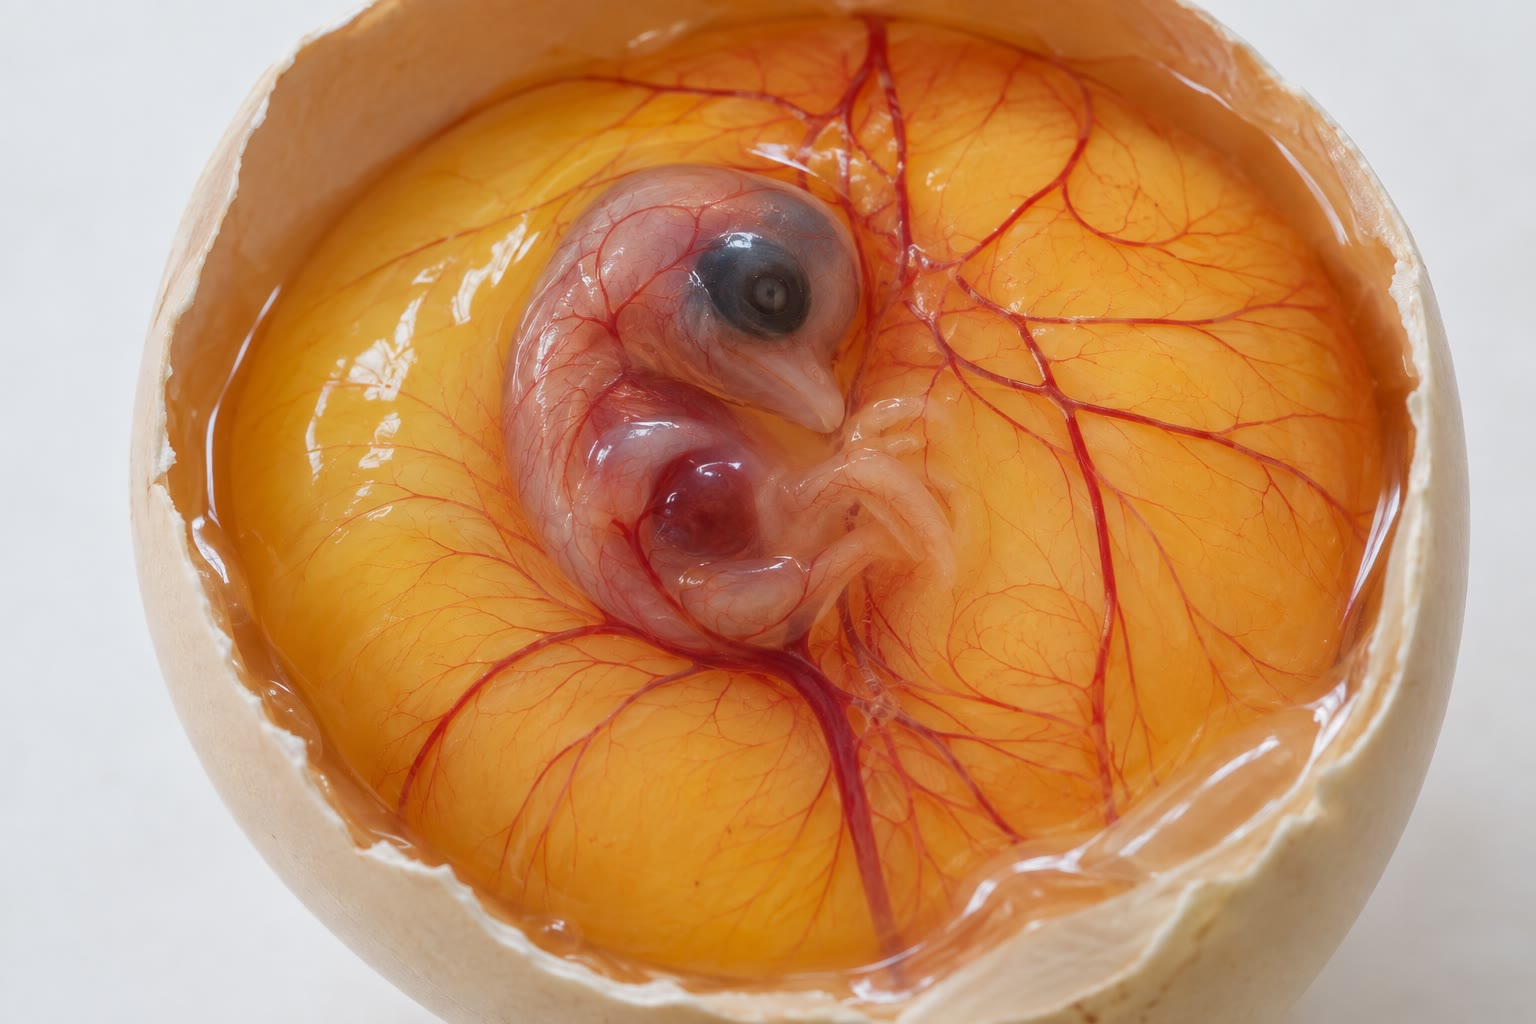
\includegraphics[width=0.5\linewidth]{images/book4/ai/b4-10-chick-embryo.jpg}

{\small Kiri: sebuah lembaga ikan zebra berumur sehari di dalam
korionnya, meringkuk mengelilingi \omterm{def:b2:vertebrate-development:egg}{kuning telurnya}, dengan mata, otak,
dan sederet somit. Kanan: sebuah lembaga anak ayam berumur tiga hari di
atas \omterm{def:b2:vertebrate-development:egg}{kuning telurnya}, jantungnya sudah berdenyut dan pembuluhnya
menyebar di atas \omterm{def:b2:vertebrate-development:egg}{kuning telurnya} untuk menyuapinya.}
\end{omfigure}

\section{Pengimbasan: bagaimana sel belajar tempatnya}

\begin{definition}[Pengimbasan dan kompetensi]\label{def:b2:vertebrate-development:induction}
\index{pengimbasan (lembaga)}\index{kompetensi}\index{pengatur}
\emph{Pengimbasan} adalah proses yang lewatnya sekelompok sel mengubah
nasib kelompok tetangganya lewat sebuah isyarat; sel yang menanggapinya
harus \emph{berkompeten} --- sanggup menjawab, dan mereka hanya sanggup
selama waktu yang terbatas. Perkembangannya adalah sebuah rantai
pengimbasan: sel tumbuhannya mengimbas mesoderm di dalam sel di
atasnya; mesoderm punggungnya --- \emph{pengatur} pada bibir
blastoporanya --- mengimbas lempeng saraf di dalam ektoderm di atasnya
lalu memolakan mesoderm di kedua sisinya; notokordnya mengimbas lantai
\omterm{prop:b2:vertebrate-development:neurulation}{tabung sarafnya}; gelembung optiknya, yaitu sebuah tunas otaknya,
mengimbas sebuah lensa di dalam kulit yang disentuhnya; lensanya
mengimbas korneanya. Tiap jaringan yang terimbas menjadi pengimbas
jaringan berikutnya. Isyaratnya adalah segelintir keluarga protein
tersekresi yang dipakai berulang-ulang --- dan keluarga yang sama pula
yang memolakan sebuah tungkai (\cref{ch:b2:limb-organogenesis}) dan,
pada dewasanya, menjalankan pengisyaratan
\cref{ch:b2:cell-signalling}.
\end{definition}
\begin{proof}[Bukti eksperimental]
Spemann dan Mangold (1924) memotong bibir blastopora punggung sebuah
gastrula dini seekor spesies kadal air lalu mencangkokkannya ke sisi
perut spesies lain, yang berpigmen berbeda sehingga sel inang dan sel
cangkokannya dapat dibedakan. Cangkokannya tidak sekadar menjadi apa
yang akan menjadi bagiannya di tempat asalnya: ia bergulir masuk,
membentuk notokord, dan \emph{mengimbas ektoderm perut inangnya
sendiri} untuk membuat sebuah \omterm{prop:b2:vertebrate-development:neurulation}{tabung saraf} kedua dan, di sebelahnya,
somit inangnya --- sebuah lembaga kedua yang lengkap, sebagian besar
dari sel inangnya, bersambung perut ke perut dengan yang pertama. Tidak
ada keping gastrula lain yang dapat melakukan hal ini. Mereka menyebut
bibirnya sebagai \omterm{def:b2:vertebrate-development:induction}{pengatur}; isyaratnya (protein yang menghadang faktor
peventralan BMP) dikenali tujuh puluh tahun kemudian.
\end{proof}

\begin{omfigure}
\begin{tikzpicture}[every node/.style={font=\scriptsize}, >=stealth]
  % donor
  \draw[thick, fill=omDef!12] (0,0) circle (1.3); \node[above] at (0,1.4) {gastrula pemberi (pucat)};
  \draw[very thick, omThm] (0.85,-0.95) arc (-45:-20:1.3); \node[omThm, right] at (1.2,-0.8) {bibir punggung};
  \draw[->, thick] (1.6,-0.3) -- (3.4,-0.3);
  % host
  \draw[thick, fill=omExo!45] (5,0) circle (1.3); \node[above] at (5,1.4) {gastrula inang (gelap)};
  \draw[very thick, omThm] (5.85,-0.95) arc (-45:-20:1.3); \node[omThm, right] at (6.2,-0.8) {bibirnya sendiri};
  \draw[very thick, omThm] (4.15,0.95) arc (135:160:1.3); \node[omThm, left] at (3.9,1.0) {cangkokan};
  \draw[->, thick] (6.6,-0.3) -- (8.4,-0.3);
  % result: twinned embryo
  \draw[thick, fill=omExo!45] (10.6,0) ellipse (1.8 and 1.1);
  \draw[very thick, omDef!70!black] (9.2,0.5) .. controls (10.0,0.8) and (11.2,0.8) .. (12.0,0.5);
  \draw[very thick, omDef!70!black] (9.2,-0.5) .. controls (10.0,-0.8) and (11.2,-0.8) .. (12.0,-0.5);
  \node[above] at (10.6,1.2) {hasilnya: dua sumbu};
  \node[anchor=north, align=center, text width=4cm] at (10.6,-1.2) {sebuah tabung saraf dan somit kedua, yang terbuat dari sel \emph{inangnya}, diimbas cangkokannya};
\end{tikzpicture}

{\small Percobaan \omterm{def:b2:vertebrate-development:induction}{pengatur}. Sebuah bibir punggung yang dicangkokkan ke
perut gastrula lain mengimbas sel inangnya untuk membentuk sumbu
lembaga kedua.}
\end{omfigure}

\begin{theorem}[Sebuah landaian morfogen]\label{thm:b2:vertebrate-development:gradient}
\index{morfogen}
Banyak pengimbasan bekerja lewat sebuah \emph{morfogen}: sebuah isyarat
yang disekresikan sebuah sumber, menyebar menembus jaringannya, lalu
dibaca sel menurut kepekatan setempatnya --- di atas satu ambang satu
nasib, di atas ambang yang lebih tinggi nasib lain. Sebuah morfogen
yang dihasilkan pada sebuah sumber bidang dengan laju $j$ tiap satuan
luas, berdifusi dengan koefisien $D$ dan terurai dengan laju $k$,
memiliki pada keadaan tunak tampang eksponensial
\[
c(x) = c_0\,e^{-x/\lambda}, \qquad \lambda = \sqrt{D/k}, \qquad c_0 = \frac{j}{\sqrt{Dk}},
\]
sehingga jarak saat kepekatannya turun di bawah sebuah ambang $T$
adalah $x_T = \lambda\ln(c_0/T)$: sebuah jaringan dapat dipolakan
menjadi pita berlebar tetap oleh ambang yang tetap. Dengan $D =
\qty{1e-12}{m^2/s}$ (sebuah protein yang diperlambat pengikatan sembari
bergerak menembus jaringannya) dan $k = \qty{1e-3}{s^{-1}}$ (waktu
paruh kira-kira dua belas menit), $\lambda = \sqrt{10^{-9}}\,\unit{m} \approx
\qty{32}{\micro m}$: yaitu beberapa garis tengah sel, skala
yang di atasnya medan lembaganya dipolakan. Melipatduakan sumbernya
melipatduakan $c_0$ lalu menggeser tiap batasnya ke luar sejauh $\lambda
\ln 2$.
\end{theorem}
\begin{proof}
Pada keadaan tunak, difusinya mengimbangi penguraiannya: $D\,c'' = k\,c$, yang penyelesaian meluruhnya adalah $c = c_0 e^{-x/\lambda}$
dengan $\lambda^2 =
D/k$. Fluks yang meninggalkan sumbernya adalah
$-Dc'(0) = Dc_0/\lambda = j$, yang memberi $c_0 = j\lambda/D = j/\sqrt{Dk}$. Menetapkan $c(x_T) = T$ memberi $x_T$; mengubah $c_0$
menjadi $2c_0$ menambahkan $\lambda\ln 2$ padanya.
\end{proof}

\begin{omfigure}
\begin{tikzpicture}
\begin{axis}[
  width=0.78\linewidth, height=5.6cm,
  axis x line=bottom, axis y line=left,
  xmin=0, xmax=120, ymin=0, ymax=1.1,
  xlabel={jarak dari sumbernya (\unit{\micro m})}, ylabel={morfogen (relatif)},
  xlabel style={font=\small, at={(axis description cs:0.5,-0.13)}, anchor=north},
  ylabel style={font=\small},
  tick label style={font=\small}, xtick={0,32,64,96}, ytick={0,0.5,1},
  clip=false,
]
\fill[omThm!18] (axis cs:0,0) rectangle (axis cs:22,1.05); \node[font=\scriptsize, anchor=south] at (axis cs:11,1.05) {nasib A};
\fill[omProp!18] (axis cs:22,0) rectangle (axis cs:61,1.05); \node[font=\scriptsize, anchor=south] at (axis cs:41,1.05) {nasib B};
\fill[omExo!18] (axis cs:61,0) rectangle (axis cs:120,1.05); \node[font=\scriptsize, anchor=south] at (axis cs:90,1.05) {nasib C};
\addplot[very thick, omDef, domain=0:120, samples=80] {exp(-x/32)};
\draw[dashed, gray] (axis cs:0,0.5) -- (axis cs:22,0.5) -- (axis cs:22,0);
\draw[dashed, gray] (axis cs:0,0.15) -- (axis cs:61,0.15) -- (axis cs:61,0);
\node[font=\scriptsize, anchor=west] at (axis cs:62,0.55) {ambang 1};
\node[font=\scriptsize, anchor=west] at (axis cs:62,0.2) {ambang 2};
\end{axis}
\end{tikzpicture}

{\small Sebuah landaian morfogen dengan $\lambda = \qty{32}{\micro m}$.
Dua ambang memotong jaringannya menjadi tiga pita nasib sel yang
lebarnya ditetapkan $\lambda$ dan rasio ambangnya terhadap kepekatan
sumbernya.}
\end{omfigure}

\begin{example}[Membaca landaiannya]\label{ex:b2:vertebrate-development:reading}
Pada gastrula katak, sel zona tepinya yang terpapar jumlah berjenjang
sebuah isyarat keluarga aktivin menjadi, dari takaran tinggi ke
rendah, notokord, otot, ginjal, dan darah; sel tudung hewan yang
dipisahkan lalu ditaruh di dalam cawan dengan takaran ambangnya
berganti nasib dalam selang faktor dua kepekatannya. Di dalam \omterm{prop:b2:vertebrate-development:neurulation}{tabung
sarafnya}, sebuah isyarat dari notokord dan lempeng lantainya menyebar
ke atas lalu menetapkan, dari bawah, neuron motorik dan kemudian
golongan interneuron berturut-turut pada ambang yang berjarak beberapa
garis tengah sel. Koordinat organismenya ditulis dalam kepekatan.
\end{example}

\section{Nasib, pemancangan, dan waktu keputusannya}

\begin{proposition}[Kapan nasib sebuah sel dipancangkan]\label{prop:b2:vertebrate-development:commitment}
\index{determinasi}\index{regulasi (lembaga)}
\emph{Nasib} sebuah sel adalah apa yang biasanya akan menjadi dirinya;
\emph{potensinya} adalah apa yang dapat menjadi dirinya kalau
dipindahkan; ia \emph{terdeterminasi} ketika nasibnya tidak lagi
berganti bersama sekelilingnya. Lembaga dini \emph{meregulasi}:
masing-masing dari kedua blastomer katak yang pertama, kalau
dipisahkan, membuat seekor berudu kecil yang utuh, dan sel pertama
sebuah lembaga mamalia semuanya totipoten --- dan begitulah kembar
identik muncul. Determinasinya datang berangsur dan pada waktu yang
berbeda bagi jaringan yang berbeda: sekeping ektoderm gastrula dini
yang dicangkokkan ke perutnya menjadi kulit perut, sedangkan keping
yang sama yang diambil dari gastrula lanjut membuat sebuah lempeng
saraf di mana pun ia ditaruh; pada tahap tunas ekornya, sebuah medan
tungkai yang dipindahkan ke sisi tubuhnya membuat sebuah tungkai di
situ. Pada sebagian besar avertebrata, sebaliknya, nasibnya dipancangkan
dini oleh sitoplasma yang diwarisi tiap selnya (perkembangan
\emph{mosaik}) dan sebuah blastomer yang dipisahkan hanya membuat
bagiannya. Siasat vertebrata --- menjaga selnya tetap lentur lalu
memberitahunya apa yang harus dikerjakan lewat pengimbasan --- itulah
yang memungkinkan pengembaran, regenerasi, dan percobaan \omterm{def:b2:vertebrate-development:induction}{pengatur}.
\end{proposition}
\begin{proof}[Bukti eksperimental]
Spemann (1901) mengikatkan sehelai gelung rambut di sekeliling sebutir
telur kadal air pada tahap dua sel: kalau gelungnya terletak pada
bidang sabit kelabunya, sehingga tiap belahannya menerima sebagiannya,
dua lembaga yang lengkap terbentuk; kalau ia terletak tegak lurus,
sehingga satu belahannya memperoleh seluruh sabitnya, belahan itu
membuat sebuah lembaga dan yang lain sebuah bola jaringan perut.
Sabitnya --- bakal \omterm{def:b2:vertebrate-development:induction}{pengaturnya} --- adalah satu-satunya bagian yang
tidak dapat dibagi dua.
\end{proof}

\begin{example}[Jadwal seekor katak]\label{ex:b2:vertebrate-development:timetable}
Pada \qty{18}{\celsius}: pembuahan; pembelahan pertama pada
\qty{1.5}{h}, lalu tiap setengah jam; \omterm{def:b2:vertebrate-development:blastula}{blastula} berisi \num{4000} sel
pada \qty{7}{h}; peralihan \omterm{def:b2:vertebrate-development:blastula}{blastula} tengah pada \qty{8}{h}; gastrulasi
\qty{10}{h} sampai \qty{20}{h}; lipatan sarafnya menutup pada
\qty{30}{h}; jantungnya berdenyut pada \qty{2.5}{d}; menetas dan makan
pada \qty{4}{d}, sebagai seekor berudu sepanjang \qty{6}{mm}. Seekor
ikan zebra melakukan hal yang sama dalam sehari, seekor anak ayam dalam
tiga hari, seekor mencit dalam sembilan hari; sebuah lembaga manusia
bergastrulasi pada pekan ketiga lalu menutup \omterm{prop:b2:vertebrate-development:neurulation}{tabung sarafnya} pada pekan
keempat --- sebelum sebagian besar perempuan tahu mereka hamil, dan
itulah sebabnya folat, yang dibutuhkan bagi penutupan \omterm{prop:b2:vertebrate-development:neurulation}{tabung sarafnya},
diresepkan sebelum pembuahan.
\end{example}

\section{Latihan}

\begin{exercise}[$\star$]\label{exo:b2:vertebrate-development:1}
Definisikan pembelahan, \omterm{def:b2:vertebrate-development:blastula}{blastula}, gastrulasi, dan neurulasi, lalu
sebutkan struktur yang dihasilkan tiap tahapnya.
\end{exercise}

\begin{exercise}[$\star$]\label{exo:b2:vertebrate-development:2}
Berikan ketiga lapisan lembaganya dan, bagi masing-masingnya, empat
jaringan dewasa yang berasal darinya.
\end{exercise}

\begin{exercise}[$\star$]\label{exo:b2:vertebrate-development:3}
Bagaimana banyaknya \omterm{def:b2:vertebrate-development:egg}{kuning telur} mengubah pola pembelahan dan pola
gastrulasinya? Bandingkan seekor katak dan seekor anak ayam.
\end{exercise}

\begin{exercise}[$\star$]\label{exo:b2:vertebrate-development:4}
Apakah pengimbasan itu? Berikan tiga pengimbasan menurut urutan
terjadinya pada sebuah lembaga katak, sambil menamai pengimbasnya dan
jaringan yang menanggapinya.
\end{exercise}

\begin{exercise}[$\star\star$]\label{exo:b2:vertebrate-development:5}
Sebutir telur katak berjari-jari \qty{1}{mm} membelah dua belas kali.
Hitunglah cacah selnya, purata jari-jarinya, dan faktor
pertumbuhan seluruh permukaan selnya. Mengapa lembaganya membutuhkan
permukaan tambahan itu?
\end{exercise}

\begin{exercise}[$\star\star$]\label{exo:b2:vertebrate-development:6}
Rasio nukleus terhadap sitoplasmanya bermula pada $10^{-4}$ dan
peralihan \omterm{def:b2:vertebrate-development:blastula}{blastula} tengahnya terjadi ketika ia mencapai $0.4$. Sesudah
berapa pembelahan? Kalau telurnya disuntik DNA sebanyak tiga kali
jumlahnya sendiri, pada pembelahan keberapa peralihannya datang?
\end{exercise}

\begin{exercise}[$\star\star$]\label{exo:b2:vertebrate-development:7}
Sebuah morfogen memiliki $D = \qty{2e-12}{m^2/s}$ dan waktu paruh
\qty{10}{min}. Hitunglah $k$ dan $\lambda$. Dua ambangnya berada pada
\qty{50}{\%} dan \qty{10}{\%} kepekatan sumbernya: berikan lebar
ketiga pita nasibnya.
\end{exercise}

\begin{exercise}[$\star\star$]\label{exo:b2:vertebrate-development:8}
Pada landaian latihan sebelumnya, sumbernya dilipatduakan sebuah
\omterm{def:b2:genome-diversification:mutation}{mutasi}. Sejauh mana tiap batasnya bergerak? Bagaimana kalau laju
penguraiannya yang dilipatduakan?
\end{exercise}

\begin{exercise}[$\star\star$]\label{exo:b2:vertebrate-development:9}
Perikanlah percobaan Spemann--Mangold, katakan mengapa kedua spesiesnya
harus berbeda pigmentasinya, lalu nyatakan apa yang disingkirkan
hasilnya.
\end{exercise}

\begin{exercise}[$\star\star\star$]\label{exo:b2:vertebrate-development:10}
Ramalkanlah hasil: (a) sekeping bakal lempeng saraf gastrula dini yang
dicangkokkan ke perutnya; (b) keping yang sama dari gastrula lanjut;
(c) sekeping ektoderm perut yang ditaruh di atas sebuah notokord pada
gastrula lanjut; (d) seluruh \omterm{def:b2:vertebrate-development:induction}{pengaturnya} dibuang dari gastrula dini.
Jelaskan masing-masingnya dengan pengertian \omterm{def:b2:vertebrate-development:induction}{kompetensi} dan
determinasi.
\end{exercise}

\begin{exercise}[$\star\star\star$]\label{exo:b2:vertebrate-development:11}
Pembelahan pertama kataknya memakan \qty{90}{min} dan sebelas
pembelahan berikutnya masing-masing \qty{30}{min}, pada
\qty{18}{\celsius}; pada \qty{10}{\celsius} tiap langkahnya 2,5 kali
lebih lambat. Pada waktu berapa peralihan \omterm{def:b2:vertebrate-development:blastula}{blastula} tengahnya tercapai
pada tiap suhunya? Jelaskan mengapa peralihannya datang pada cacah sel
yang sama pada kedua suhunya, dan apa yang dikatakannya tentang jamnya.
\end{exercise}

\begin{exercise}[$\star\star\star$]\label{exo:b2:vertebrate-development:12}
``Sebuah lembaga vertebrata dibangun lewat percakapan, sebuah lembaga
avertebrata lewat pewarisan.'' Bahaslah pertentangan antara
perkembangan regulatif dan mosaik, akibatnya bagi pengembaran dan
regenerasi, serta mengapa ia adalah perbedaan derajat.
\end{exercise}

\section{Soal: Sebuah Lembaga Katak Diwaktui dan Dipolakan}

\begin{problem}[{Soal akhir pekan --- sebuah lembaga katak diikuti
melalui pembelahan, peralihan blastula tengah, gastrulasi, dan
pengimbasan, dengan landaian morfogennya dihitung dan cangkokan
klasiknya diramalkan, berakhir pada cacah sel dan waktu peralihannya
serta lebar pita nasibnya}]
\label{pb:b2:vertebrate-development:1}
Sebutir telur katak berjari-jari \qty{0.7}{mm} dan bernukleus
berjari-jari \qty{0.03}{mm} yang kandungan DNA-nya $c$; tiap pembelahan
memakan \qty{30}{min} sesudah pembelahan pertama \qty{75}{min}.
Peralihan \omterm{def:b2:vertebrate-development:blastula}{blastula} tengahnya terjadi ketika seluruh DNA-nya mencapai
$4000\,c$. Morfogennya: $D =
\qty{1e-12}{m^2/s}$, waktu paruh
\qty{20}{min}, kepekatan sumbernya $c_0$, ambangnya pada $0.4\,c_0$ dan
$0.08\,c_0$.

\medskip
\noindent\textbf{Bagian I --- Pembelahannya.}
\begin{enumerate}
  \item Hitunglah volume telurnya dan volume nukleusnya, serta rasio
        awal nukleus terhadap sitoplasmanya.
  \item Sesudah berapa pembelahan DNA-nya mencapai $4000\,c$? Berapa
        selnya?
  \item Pada waktu berapa sesudah pembuahannya?
  \item Berapa purata jari-jari selnya saat itu, dan berapa rasio
        volume nukleus terhadap volume selnya kalau nukleusnya
        mempertahankan ukurannya? Berilah ulasan.
  \item Dengan faktor berapa seluruh permukaan selnya telah tumbuh?
  \item Tiap pembelahannya menuntut genomnya disalin: berapa banyak DNA
        yang telah disintesis seluruhnya, dalam satuan $c$, dan mengapa
        lembaganya tidak perlu mentranskripsi gennya untuk itu?
  \item Apa yang berubah pada peralihannya, dan percobaan apa yang
        menunjukkan bahwa ia dipicu sebuah rasio dan bukan sebuah
        cacahan?
\end{enumerate}

\medskip
\noindent\textbf{Bagian II --- Gastrulasinya.}
\begin{enumerate}[resume]
  \item Di manakah blastopornya terbentuk relatif terhadap titik masuk
        spermanya, dan apa yang memancangkan kedudukan itu?
  \item Daftarkan, menurut urutannya, jaringan yang bergulir masuk
        lewat blastopornya dan kedudukannya sesudah itu.
  \item Gastrulasinya memakan \qty{10}{h} dan lembaran yang berinvolusi
        menempuh \qty{2}{mm}. Hitunglah purata kelajuan selnya dalam
        mikrometer tiap menit lalu bandingkan dengan sebuah fibroblas
        yang merangkak (\qty{1}{\micro m/min}).
  \item Mengapa gastrulasi mustahil sebelum peralihan \omterm{def:b2:vertebrate-development:blastula}{blastula}
        tengahnya?
  \item Jelaskan dalam satu kalimat mengapa notokordnya, dan bukan
        \omterm{prop:b2:vertebrate-development:neurulation}{tabung sarafnya}, yang menjadi struktur penentu kordata.
  \item Sebuah obat yang menghadang pergantian bentuk sel diberikan
        pada awal gastrulasinya. Ramalkanlah lembaganya.
\end{enumerate}

\medskip
\noindent\textbf{Bagian III --- Landaiannya.}
\begin{enumerate}[resume]
  \item Hitunglah $k$ dari waktu paruhnya, dan $\lambda$.
  \item Hitunglah kedudukan kedua ambangnya.
  \item Berikan lebar ketiga pita nasibnya dalam mikrometer dan dalam
        sel berukuran \qty{15}{\micro m}.
  \item Sumbernya dijadikan separuh. Hitunglah kembali kedua
        kedudukannya lalu nyatakan pita mana yang paling menyusut.
  \item Sebuah sel berjarak \qty{60}{\micro m} dari sumbernya
        dipindahkan ke \qty{10}{\micro m} sebelum landaiannya dibaca;
        lalu sesudahnya. Menjadi apa ia pada tiap kasusnya, dan mengapa?
  \item Jelaskan mengapa tampang eksponensial memberi batas yang
        kedudukannya bergantung pada logaritma kekuatan sumbernya, dan
        mengapa hal ini membuat pemolaannya tegar.
\end{enumerate}

\medskip
\noindent\textbf{Bagian IV --- Cangkokannya.}
\begin{enumerate}[resume]
  \item Ramalkanlah hasil mencangkokkan sebuah bibir punggung ke sisi
        perut sebuah gastrula dini, dan hasil mencangkokkan zona tepi
        perut ke sisi punggungnya.
  \item Ramalkanlah hasil mencangkokkan sebuah bibir punggung ke sisi
        perut sebuah \emph{neurula}, lalu jelaskan perbedaannya.
  \item Sebuah lembaga katak pada tahap dua sel dibelah sepanjang
        bidang sabit kelabunya; lembaga lain dibelah tegak lurus
        terhadapnya. Ramalkanlah keduanya.
  \item Sebuah tudung hewan dipotong dari sebuah \omterm{def:b2:vertebrate-development:blastula}{blastula} lalu dibiakkan
        sendirian; tudung yang sama dibiakkan di sebelah sel
        tumbuhannya. Ramalkanlah jaringan yang terbentuk.
  \item Mengapa hasil Spemann dan Mangold menuntut inang dan
        cangkokannya dapat dibedakan, dan apa yang akan ditunjukkan
        sebuah cangkokan dari spesies yang keliru?
  \item Nyatakan hasilnya: cacah pembelahan dan waktu peralihannya,
        cacah selnya, dan ketiga lebar pitanya.
\end{enumerate}
\end{problem}
